% !TeX program = lualatex
\documentclass[aspectratio=169]{beamer}
\usepackage{fontspec}
\usepackage{animate}
\usepackage{booktabs}
\usepackage{amsmath}
\usepackage{amsfonts}
\usepackage[url=false, doi=false]{biblatex}
\addbibresource{ref.bib}
\usetheme{YSbeamer}
\usepackage{graphicx}
\usepackage{adjustbox}
\usepackage{subcaption}
% \usepacksubsection nameoverlay]{textpossubsection namef{#1}}}
\newcommand{\vect}[1]{{\mathbf{#1}}}

\usefonttheme{professionalfonts} % using non standard fonts for beamer
\usefonttheme{serif} % default family is serif
\usepackage{fontspec}
\setmainfont{Avenir}

\title{Data assimilation with ML for parameter}
\author{Yixuan Sun}

\begin{document}

\begin{frame}{Preconditioners}
    The general idea of preconditioning~(in Krylov subspace method) is to reduce the spectral \textbf{condition number} in the coefficient matrix so that it can be solved more efficiently~(faster convergence).
    \begin{equation}\label{eqn:linear-sys}
        A\vect{x} = \vect{b}
    \end{equation}
    The condition number of a matrix $A$ is 
    \begin{equation}\label{eqn:condition-number}
        \kappa(A) = \Vert A \Vert_2 \Vert A^{-1} \Vert_2,
    \end{equation}
    With preconditioner $P$,
    \begin{equation}
        P^{-1}A\vect{x} = P^{-1}\vect{b}
    \end{equation}
    An iteration 
    \begin{equation}
        \vect{x}_{k+1} = \vect{x}_{k} + P^{-1}(\vect{b} - A\vect{x}_{k})
    \end{equation}
\end{frame}

% \begin{frame}{Conjugate Gradient Method}
%     We talk about the CG~(a kind of iterative method) can benefit from preconditioners. CG works with (sparse) systemtric postiive definite~(SPD) systems.  
    
% \end{frame}

\begin{frame}{Types of preconditioners}
   \begin{itemize}
    \item Jacobi
    \item Gauss-Seidel
    \item Incomplete LU~(ILU)
    \item Algebraic Multigrid~(AMG) 
   \end{itemize} 
   \vspace{1em}
   Jacobi, Gauss-Seidel quickly get rid of high frequency errors but slow reduction on low frequency errors. ILU and AMG can serve as more general preconitioners.

   Due to its flexibility and popularity, we chose to generate AMG preconditioners for linear systems.
\end{frame}

\begin{frame}{Data Generation}
    We focus on symmetric positive definite matrices to serve Conjugate Graident~(CG) method
    \begin{figure}
        \centering
        \begin{subfigure}{0.3\textwidth} 
            \centering
            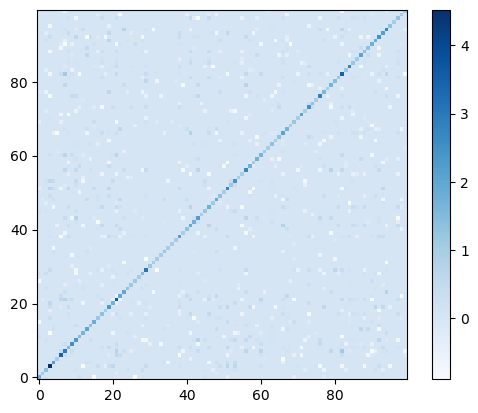
\includegraphics[width=\linewidth]{./figures/example_SPD_matrix.png}
            \caption{Original system $A$}
        \end{subfigure}
        \begin{subfigure}{0.3\textwidth} 
            \centering
            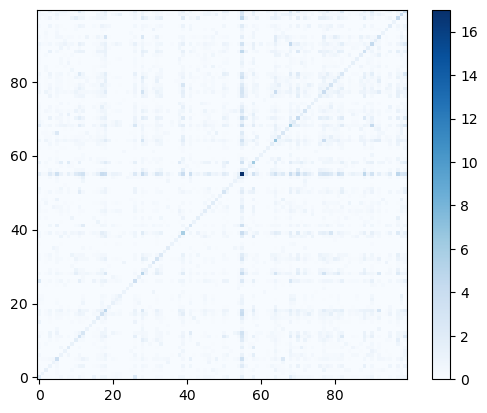
\includegraphics[width=\linewidth]{./figures/example-ILU.png}
            \caption{ILU preconditioner}
        \end{subfigure}
        \begin{subfigure}{0.3\textwidth} 
            \centering
            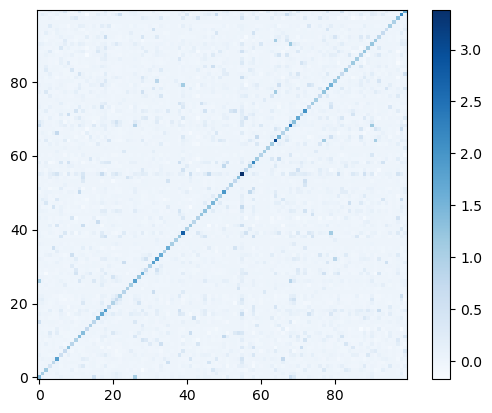
\includegraphics[width=\linewidth]{./figures/example-amg.png}
            \caption{AMG preconditioner}
        \end{subfigure}
        \caption{Example linear system and its ILU and AMG preconditioners.}
        \label{fig:spd_mat}
    \end{figure}
\end{frame}

\begin{frame}{Model training}
   We can train ML models with (1) unsupervised objectives, encouraging the resulting matrix to lower the condition number of the system while staying close to the original; (2) supervised objectives, learning to predict the pre-generated preconditioners. 
   \vspace{1em}
   \begin{columns}
        \begin{column}[t]{.5\textwidth}
            Unsupervised loss
            \begin{equation}
                \begin{aligned}
                    &L_{\kappa} = \Vert M^{-1}A \Vert_2 \Vert (M^{-1}A)^{-1}\Vert_2\\
                    &L_{inv} = \frac{1}{1 + \vert \text{det}(M)\vert}\\
                    &L_{approx}  = \Vert A - M \Vert_p\\
                    &Loss = \alpha L_{\kappa} + \beta L_{inv} + \gamma L_{approx}
                \end{aligned}
            \end{equation}
        \end{column}
        \begin{column}[t]{.5\textwidth}
            Supervised loss
            \begin{equation}
                L = \Vert M - M_{true}\Vert_2^2
            \end{equation}
            
        \end{column}
   \end{columns}
\end{frame}

\begin{frame}{Preliminary Results}

    \begin{columns}
        \begin{column}[t]{.5\textwidth}
            Supervised 

            \begin{figure}
                \centering
                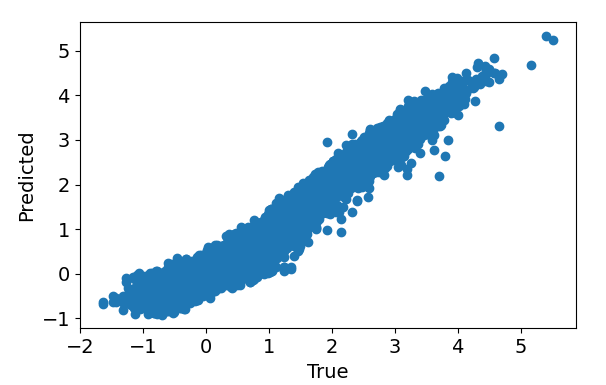
\includegraphics[width=\linewidth]{./figures/scatter_UNET_amg.png}
                \caption{True vs. Predicted scatter plot on the testing set. $R^2 = 0.86$, $MAPE = 0.58$}
            \end{figure}   
        \end{column}
        \begin{column}[t]{.5\textwidth}
            Unsupervised
            \begin{figure}
                \centering
                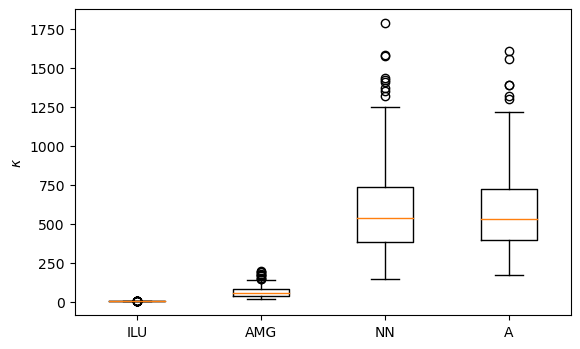
\includegraphics[width=\linewidth]{./figures/kappa-boxplot.png}
                \caption{Boxplot of the condition number of different preconditioned system and the original.}
            \end{figure}
        \end{column}
    \end{columns}
\end{frame}

\begin{frame}{Preliminary Results}
    \begin{itemize}
        \item The supervised scheme shows better performance. However, the accuarcy needs to be drastically improved for the subsequent solver.
        \item  Since the choice of preconditioners highly depends on the problem and the structure of the coefficient matrix, we would like to exploit problem-specific knowledge during learning.
        \item Moreover, we can break down the end-to-end pipeline into different parts~(based on the corresponding numerical method) and utilize separate models for them to improve results.
    \end{itemize}
\end{frame}
\end{document}